\documentclass[sigconf,nonacm]{acmart}
\usepackage{booktabs}
\usepackage{tikz}
\emergencystretch=1.5em
\setcopyright{none}
\settopmatter{printacmref=false}
\renewcommand\footnotetextcopyrightpermission[1]{}
\begin{document}
% Resolve numeric citations on the editor compiler's first pass; aux labels take precedence on later passes.
\makeatletter
\@ifundefined{b@pizzorno2025coverup}{\bibcite{pizzorno2025coverup}{1}}{}
\@ifundefined{b@renodetime}{\bibcite{renodetime}{2}}{}
\@ifundefined{b@banik2026}{\bibcite{banik2026}{3}}{}
\@ifundefined{b@barr2015oracle}{\bibcite{barr2015oracle}{4}}{}
\@ifundefined{b@berndt2026}{\bibcite{berndt2026}{5}}{}
\@ifundefined{b@chen2024chatunitest}{\bibcite{chen2024chatunitest}{6}}{}
\@ifundefined{b@dakhel2024mutap}{\bibcite{dakhel2024mutap}{7}}{}
\@ifundefined{b@aim2023}{\bibcite{aim2023}{8}}{}
\@ifundefined{b@embctest2026}{\bibcite{embctest2026}{9}}{}
\@ifundefined{b@jia2011mutation}{\bibcite{jia2011mutation}{10}}{}
\@ifundefined{b@luo2014flaky}{\bibcite{luo2014flaky}{11}}{}
\@ifundefined{b@rahman2024flakerake}{\bibcite{rahman2024flakerake}{12}}{}
\@ifundefined{b@regehr2005random}{\bibcite{regehr2005random}{13}}{}
\@ifundefined{b@stm32f407datasheet}{\bibcite{stm32f407datasheet}{14}}{}
\@ifundefined{b@strandberg2020}{\bibcite{strandberg2020}{15}}{}
\@ifundefined{b@aidfuzzer2025}{\bibcite{aidfuzzer2025}{16}}{}
\@ifundefined{b@sdracer2017}{\bibcite{sdracer2017}{17}}{}
\@ifundefined{b@embedagent2026}{\bibcite{embedagent2026}{18}}{}
\@ifundefined{b@zephyrpinned}{\bibcite{zephyrpinned}{19}}{}
\makeatother


\title[Clock Robustness and Alarm Precision]{Clock Robustness and Alarm Precision in LLM-Generated and Upstream Zephyr RTC Tests}
\author{Pranav Krishnan}
\affiliation{\institution{The University of Texas at Austin}\city{Austin}\state{Texas}\country{USA}}
\author{Keshav Bhargava}
\affiliation{\institution{The University of Texas at Austin}\city{Austin}\state{Texas}\country{USA}}

\begin{abstract}
Deterministic reruns can miss a firmware test's unjustified timing bound. We compared selected human-written upstream Zephyr real-time clock (RTC) tests and functionally eligible LLM-generated suites under datasheet-legal oscillator settings and separate alarm faults. The three upstream cases failed at 17--26 of 100 sampled legal settings; all 37 measured LLM failures came from three range-absent pending suites. The suite-level prompt contrast, 3/24 absent versus 0/26 present, was not significant. In a task-specific alarm-offset probe, evaluable generated callback suites detected 18/18 early and 14/18 late faults, while one upstream callback case detected neither; the LLM specification explicitly requested configured-time firing. Clock robustness, generation yield, and oracle precision require separate assessment.
\end{abstract}
\keywords{embedded testing, flaky tests, interrupt-driven firmware, RTC, large language models}
\maketitle

\section{Introduction}
A real-time clock (RTC) alarm test may schedule an event ten calendar seconds ahead, wait thirteen host seconds, and assert that a callback arrived. The assertion is valid only if thirteen seconds accommodates the RTC clock and delivery path. Repeating the same simulator schedule cannot test that premise. Changing the oscillator within its documented range can change the verdict without changing test or firmware source.

We call the selected human-written Zephyr cases \emph{upstream tests}. We compare their clock sensitivity with LLM-generated tests and then challenge surviving tests with faults that separate clock tolerance from alarm-oracle precision. The upstream cases were chosen for visible timing windows, not sampled to represent Zephyr generally. We ask: \textbf{RQ1}, which tests flip under legal clock settings? \textbf{RQ2}, which faults do they detect? \textbf{RQ3}, how accurately does a static threshold predict flips, and for which tests? \textbf{RQ4}, which source-level timing assumptions remain? We contribute a frozen paired clock schedule, prospective threshold validation, replay and reference triage, all-attempt generation accounting, and task-matched fault probes. Sampled-setting shares below are simulation sensitivities, not field failure probabilities.

\section{Approach}
\textbf{Clock model.} The pinned Zephyr revision~\cite{zephyrpinned} supplies upstream alarm-callback, alarm-pending, and calendar-counting cases. The STM32F4 Discovery board definition selects the low-speed internal oscillator (LSI) as the RTC source. At 3 V across $-40$ to $105\,^{\circ}$C, the STM32F407 datasheet characterizes LSI at 17--47 kHz~\cite{stm32f407datasheet}. With the build's fixed $128\times250$ prescaler, ten RTC seconds ideally take $t(f)=320{,}000/f$ host seconds: 6.809 s at 47 kHz and 18.824 s at 17 kHz. The input-clock range does not bound interrupt-delivery latency.

\textbf{Threshold forecast.} For tests with a scalar observation window, the ideal model predicts a failure when $320{,}000/f$ exceeds that window. Forecasts were frozen before clock-variation runs; tests whose callback ordering or polling prevents a scalar bound have no such prediction.

\textbf{Fault probes.} We test out-of-spec fast and slow oscillator inputs, a nominal-frequency \emph{nonarrival fault} that suppresses callback/pending delivery or freezes counting reads, and separate nominal-clock driver faults that shift the alarm compare by $-1$ or $+1$ RTC second. A \emph{kill} requires an activated fault and an explicit failure of the selected test case.

\section{Experimental Setup}

\textbf{Models, prompts, and gates.} The model IDs \texttt{gpt-6-luna}, \texttt{gpt-6-sol}, and \texttt{gpt-6-astra} (Luna, Sol, and Astra below) each returned five independent, source-only C tests using ztest (Zephyr's test framework) for 13 tasks under two prompt conditions: 390 generations. A \emph{range-absent} prompt omits numeric oscillator limits; a \emph{range-present} prompt adds low-speed and high-speed internal oscillator (HSI) ranges plus a callback-delivery reminder. The other ten tasks address narrower HSI timing effects; this analysis focuses on the three RTC tasks because the legal LSI range and alarm fault probes apply to them. The models could not build, run, or revise tests from feedback. Functional review, build, and five nominal passes defined eligibility; timing-bound adequacy was measured separately. Across all 13 tasks, 330/390 passed functional review and 321/390 passed nominal screening. The RTC analysis covers 90 attempts and 66 eligible suites.

% Source: generated/spec_context_factorial_v1/prompts/rtc_alarm_callback/range_absent.txt and rtc_alarm_pending/range_absent.txt
The frozen callback and pending prompts state these \emph{Required observable checks}, respectively:
\begin{quote}\small
``Neither callback is observed before the alarm time. Both callbacks fire at the configured RTC time and report the expected alarm IDs. The test checks callbacks through observable events or protected state and applies a finite, justified bound.''
\end{quote}
\begin{quote}\small
``The test configures and reads back a supported RTC alarm time successfully. The alarm is not observed pending before its configured RTC time. The alarm is observed pending after the RTC reaches its configured time, under a finite, justified observation bound.''
\end{quote}

\textbf{Schedule and attribution.} Each measured suite ran in a fresh Renode process (an instruction-level embedded simulator)~\cite{renodetime} at 100 shared, uniformly sampled integer LSI settings and both endpoints. ELF, source, CPU, SysTick, and synchronization quantum were fixed. The arm measured all 36 suites without a scalar clock prediction and a balanced sample of 14 of the 30 predictable suites; 16 remain forecast only. Assertion flips were classified using saved traces, source boundaries, same-input replays, and task-specific references that check premature behavior and wait under a 26-second experimental ceiling. Ambiguous, firmware, simulator, and harness outcomes remain separate. At nominal host settings, all 66 eligible generated suites and three upstream cases faced the oscillator and nonarrival probes; 39 generated and two upstream alarm cases faced the signed alarm offsets. Twenty-seven generated and one upstream counting case were non-activation controls. The task is the primary comparison unit; the registered prompt contrast subtracts absent from present rates within model and task, then averages tasks and models equally. Missing verdicts and forecasts are never recoded as observed passes. The fault probes, alarm-offset probes, and all-attempt, paired, and similarity analyses were added after varied-clock runs began; the dated amendment log is in the repository.

\begin{figure}[t]
\centering
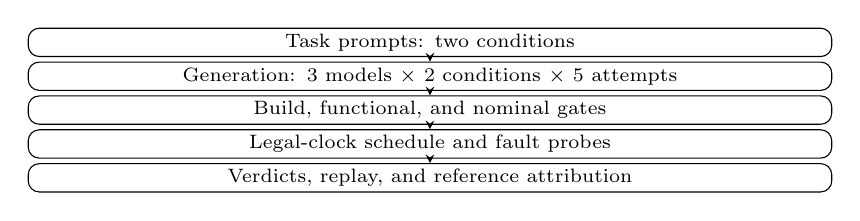
\begin{tikzpicture}[>=stealth, every node/.style={draw, rounded corners, align=center, font=\scriptsize, text width=0.83\columnwidth, inner sep=2pt}]
\node (p) at (0,0) {Task prompts: two conditions};
\node (g) at (0,-0.43) {Generation: 3 models $\times$ 2 conditions $\times$ 5 attempts};
\node (e) at (0,-0.86) {Build, functional, and nominal gates};
\node (v) at (0,-1.29) {Legal-clock schedule and fault probes};
\node (a) at (0,-1.72) {Verdicts, replay, and reference attribution};
\draw[->] (p.south)--(g.north);
\draw[->] (g.south)--(e.north);
\draw[->] (e.south)--(v.north);
\draw[->] (v.south)--(a.north);
\end{tikzpicture}
\caption{Evaluation pipeline for each RTC task. Generated sources pass eligibility gates before clock and fault challenges.}
\Description{Five vertically linked stages show prompts, generation, gates, challenges, and attributed verdicts.}
\label{fig:pipeline}
\end{figure}

\section{Results}
\subsection{Legal-clock flips (RQ1)}
A fixed observation window $T$ has an ideal failure boundary $f<320/T$ kHz. Its analytic failing fraction over a continuous uniform 17--47 kHz interval is $\max(0,\min(1,(320/T-17)/30))$. Table~\ref{tab:human} compares these fractions with the registered samples. Small differences reflect finite integer-frequency sampling; counting uses an approximate last-poll boundary.

\begin{table}[t]
\caption{Upstream legal-LSI thresholds and sampled failures.}
\label{tab:human}\scriptsize
\begin{tabular}{@{}lrrr@{}}\toprule
Case & Boundary & Analytic & Sampled \\ \midrule
Callback & 24.615 kHz & 25.38\% & 26/100 \\
Counting & 22.069 kHz & 16.90\% & 17/100 \\
Pending & 24.615 kHz & 25.38\% & 26/100 \\
\bottomrule\end{tabular}
\end{table}

\begin{figure}[t]
\centering
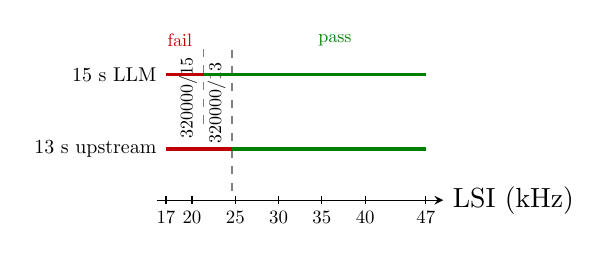
\begin{tikzpicture}[x=0.11cm,y=0.59cm,>=stealth]
\draw[->] (16,0) -- (49,0) node[right] {LSI (kHz)};
\foreach \x in {17,20,25,30,35,40,47} {\draw (\x,0.09)--(\x,-0.09) node[below,scale=.68] {\x};}
\draw[dashed,gray] (24.62,0.2)--(24.62,3.25);
\node[scale=.65,rotate=90,anchor=south] at (24.62,2.1) {$320000/13$};
\draw[very thick,red!75!black] (17,1.1)--(24.62,1.1);
\draw[very thick,green!50!black] (24.62,1.1)--(47,1.1);
\node[anchor=east,scale=.72] at (16.7,1.1) {13 s upstream};
\draw[dashed,gray] (21.33,1.65)--(21.33,3.25);
\node[scale=.65,rotate=90,anchor=south] at (21.33,2.2) {$320000/15$};
\draw[very thick,red!75!black] (17,2.7)--(21.33,2.7);
\draw[very thick,green!50!black] (21.33,2.7)--(47,2.7);
\node[anchor=east,scale=.72] at (16.7,2.7) {15 s LLM};
\node[scale=.65,red!75!black] at (18.6,3.45) {fail};
\node[scale=.65,green!50!black] at (36.5,3.45) {pass};
\end{tikzpicture}
\caption{Computed ideal-clock pass/fail steps for a 13-second upstream window and a representative 15-second LLM window. A test fails when $320000/f$ exceeds its window. The registered per-seed forecasts and observed vectors, not this schematic, determine the reported counts.}
\Description{Two horizontal frequency steps turn from failure to pass at about 24.62 and 21.33 kilohertz for upstream and representative LLM windows.}
\label{fig:step}
\end{figure}

Across the 53 measured suites, including upstream controls, 5,300 seeded originals yielded 5,182 passes, 106 assertion failures, and 12 harness errors. All 112 seeded-plus-endpoint assertion failures reproduced in persisted replay fields. References passed 3/3 nominal controls, 6/6 endpoints, and 69/69 distinct failing-setting challenges; source boundaries and traces classify all 112 as brittle test assumptions. The 12 errors stay missing.

All 37 generated-suite failures came from three range-absent pending suites: Sol r01 (11), Sol r03 (13), and Astra r05 (13). Their full forecast vectors matched. Measured range-absent suites had 37 failures in 2,400 seed slots, with four missing; range-present suites had zero in 2,600, with eight missing. At suite level, 3/24 absent versus 0/26 present flipped (two-sided Fisher $p=0.103$). Table~\ref{tab:agent} keeps measured and forecast-only suites distinct.

\begin{table}[t]
\caption{Generated RTC clock outcomes by model and prompt. A/P denote range absent/present. Failures use evaluable measured seeds.}
\label{tab:agent}\scriptsize
\begin{tabular}{@{}llrrr@{}}\toprule
Model & Prompt & Eligible & Measured & Fail/evaluable \\ \midrule
Luna & A & 4 & 2 & 0/200 \\
Luna & P & 3 & 2 & 0/200 \\
Sol & A & 15 & 11 & 24/1096 \\
Sol & P & 15 & 13 & 0/1292 \\
Astra & A & 15 & 11 & 13/1100 \\
Astra & P & 14 & 11 & 0/1100 \\
\bottomrule\end{tabular}
\end{table}

The registered present-minus-absent task contrasts are Sol callback $-0.2$ to $+1.2$, counting zero, pending $-5.4$ to $-4.4$ percentage points; Astra callback/counting zero, pending $-2.6$; and Luna counting zero. Equal-task averages are Sol $-1.87$ to $-1.07$, Astra $-0.87$, and Luna zero points; the equal-model average is $-0.91$ to $-0.64$. Hybrid bounds combine measured verdicts with 16 frozen forecasts for unrun suites and bracket missing outcomes as passes or failures; they are not fully measured rates. Suite-weighted sensitivity and missing-outcome details are in the repository's analysis materials.

\subsection{Paired comparisons on the registered settings}
% Source: analysis/rtc_stage_a_quant.json, mcnemar_per_suite
Each measured generated suite was compared with its matched upstream case on identical evaluable frequencies. Exact per-suite McNemar tests gave $p<0.05$ for 19/19 callback, 20/20 pending, and 11/11 counting suites. Upstream-fail/generated-pass discordances totaled 492, 480, and 187 by task; no evaluable pair had the reverse discordance. Seven callback and five pending seed pairs with missing generated verdicts were omitted. The 50 suites reuse the same settings and share only three task families, so these tests describe this schedule rather than 50 independent replications.

\subsection{Fault detection (RQ2)}
The ideal legal ten-second alarm-arrival window is 6.809--18.824 host seconds. The 64-kHz oscillator reaches the target at 5.000 s; the 10-kHz oscillator reaches it at 32.000 s. The fast-clock probe needs an independent time reference, whereas the alarm-offset probes change the compare relative to the nominal RTC calendar. Every selected upstream and generated suite survived the fast oscillator. Slow-fault and nonarrival kills are in Table~\ref{tab:faults}; the one missing Luna nonarrival original is unscored. Over-padding mattered: 0/12 suites with a scalar budget above twice the legal slow bound killed the slow fault, versus 18/18 at or below twice the bound. By wait style, slow-fault kills were 39/53 for fixed-sleep-only tests, 7/9 for event-wait-only tests, and 3/4 for mixed tests (tabulations in the repository's analysis directory).



\begin{table*}[t]
\caption{Out-of-spec oscillator and nonarrival kills at nominal host timing, with descriptive 95\% Wilson intervals. One Luna absent nonarrival original is missing.}
\label{tab:faults}
\small
\begin{tabular}{@{}llrrr@{}}
\toprule
Model & Range & Fast oscillator & Slow oscillator & Nonarrival \\
\midrule
Upstream & n/a & 0/3 [0, 56.1]\% & 3/3 [43.9, 100]\% & 3/3 [43.9, 100]\% \\
Luna & absent & 0/4 [0, 49.0]\% & 4/4 [51.0, 100]\% & 3/3 [43.9, 100]\% +1 missing \\
Luna & present & 0/3 [0, 56.1]\% & 0/3 [0, 56.1]\% & 3/3 [43.9, 100]\% \\
Sol & absent & 0/15 [0, 20.4]\% & 13/15 [62.1, 96.3]\% & 15/15 [79.6, 100]\% \\
Sol & present & 0/15 [0, 20.4]\% & 9/15 [35.7, 80.2]\% & 15/15 [79.6, 100]\% \\
Astra & absent & 0/15 [0, 20.4]\% & 9/15 [35.7, 80.2]\% & 15/15 [79.6, 100]\% \\
Astra & present & 0/14 [0, 21.5]\% & 14/14 [78.5, 100]\% & 14/14 [78.5, 100]\% \\
\midrule
All LLM & both & 0/66 [0, 5.5]\% & 49/66 [62.6, 83.3]\% & 65/65 [94.4, 100]\% +1 missing \\
\bottomrule
\end{tabular}
\end{table*}

At nominal clock, the upstream callback killed neither signed one-RTC-second alarm offset, whereas generated callback suites killed 18/18 evaluable early and 14/18 late. The pending task is readback-heavy by specification: all 20 generated pending suites killed both signs; upstream pending killed late, while its early original had no verdict. All 56 counting-control runs passed without alarm programming. Of 73 activated kills, 72 first failed a programmed-compare or calendar-relative check; one composite flag had an unresolved immediate cause. % Sources: generated/spec_context_factorial_v1/suites/sol/range_absent/rtc_alarm_callback/r01/test.c and r02/test.c; range_present/r01/test.c and r05/test.c
The four late-offset survivors were Sol range-absent callback r01 and r02, whose final assertions accept RTC second 5 \emph{or} 6, and Sol range-present callback r01 and r05, which lack an upper calendar-time bound. r05 additionally allows a 60-second deadline. Missing originals are never replaced by diagnostic reruns.

\begin{table}[t]
\caption{Alarm-offset kills by matched task at nominal clock, with descriptive 95\% Wilson intervals for generated suites. Missing originals are excluded.}
\label{tab:offset}\scriptsize
\begin{tabular}{@{}lrr@{}}\toprule
Case & $-1$ RTC s & $+1$ RTC s \\ \midrule
Upstream callback & 0/1 & 0/1 \\
Generated callback & 18/18 [82.4, 100]\% & 14/18 [54.8, 91.0]\% \\
Upstream pending & missing & 1/1 \\
Generated pending & 20/20 [83.9, 100]\% & 20/20 [83.9, 100]\% \\
\bottomrule\end{tabular}
\end{table}

\subsection{Prediction and generation yield (RQ3)}
A clock-only threshold applied to 30/66 eligible RTC suites. Eleven of 14 sampled predictable suites had zero-failure forecasts with budgets above the legal slow-arrival bound. The three nontrivial forecasts matched exact 100-setting vectors, including 37/37 failures; agreement across the full sample was 1,400/1,400. The other 16 predictable suites remain unrun forecasts. The frozen forecast ledger in the repository's analysis directory records their budgets.

Across all 90 RTC attempts, 15 failed to build, eight failed the functional gate, and one failed nominal screening. Thirty-nine attempts produced a confirmed clock-robust test; 29 also killed the slow and nonarrival faults. A stricter source-coded criterion requiring a known, non-over-padded clock budget admitted 5/90. Table~\ref{tab:yield} preserves the condition-level denominator. Luna had no eligible alarm suite; its range-present counting suites used 60-second windows and all missed the slow fault. Sol had two clock-flipping pending suites and weaker slow-fault detection with the range; Astra had one flipping pending suite and 14/14 range-present slow-fault kills. Between-model Fisher tests are exploratory because the three tasks share a driver and emulator.

\begin{table}[t]
\caption{All-attempt RTC yield. Each row contains 15 generation attempts. Robust means 100 observed legal-clock passes without missing verdicts; +2 also kills slow and nonarrival faults.}
\label{tab:yield}\scriptsize
\begin{tabular}{@{}llrrr@{}}\toprule
Model & Prompt & Working & Robust & Robust+2 \\ \midrule
Luna & A & 4/15 & 2/15 & 2/15 \\
Luna & P & 3/15 & 2/15 & 0/15 \\
Sol & A & 15/15 & 6/15 & 5/15 \\
Sol & P & 15/15 & 8/15 & 3/15 \\
Astra & A & 15/15 & 10/15 & 8/15 \\
Astra & P & 14/15 & 11/15 & 11/15 \\
\bottomrule\end{tabular}
\end{table}

\subsection{Reference timing and upstream source patterns}
% Sources: analysis/rtc_stage_a_reference_durations.csv and analysis/rtc_stage_a_upstream_patterns.csv
At 28 measured callback-reference frequencies, ztest duration minus $320000/f$ ranged from $-0.001$ to $+0.127$ s; this supports Renode's internal timing, not silicon fidelity. Among 33 scanned upstream RTC, counter, and timer files, none explicitly measured interrupt-to-callback latency against a registered bound.

\subsection{Supporting source review (RQ4)}
A single unblinded automated review flagged latency or ordering assumptions in 28/66 eligible RTC suites; 24 were unknown and 14 had no flagged pattern. Among 47 measured suites without clock-induced assertion failures, 21 had a definite latency premise and 23 were unknown. The three selected upstream RTC files were marked as clock-bound shortfalls in the 33-file scan.

\subsection{Source similarity to upstream}
% Sources: analysis/rtc_stage_a_similarity.json and analysis/rtc_stage_a_oracle_assertions.csv
A rule-based audit compared all 90 generated RTC sources with matched upstream tests across assertion types, fault profiles, API calls, and token overlap. The maximum pairwise five-token Jaccard score was 0.131, flagging no near-copy under this metric but not ruling out smaller reused fragments or training exposure.

\section{Discussion and Threats to Validity}
The selected upstream callback checks absence after one fixed sleep and occurrence after another. By contrast, an Astra generated callback captures RTC calendar time and asserts equality with the requested target second. Figure~\ref{fig:sourcecontrast} shows the source excerpts. The former accepts either alarm offset; the latter kills both. This is an illustrative, task-matched contrast: the generated prompt asked for configured-time firing, while Zephyr's upstream tests run across many boards and drivers where a lenient window may support portability. The pending prompt expressly required readback, so its kills mainly show instruction-following. Still, four generated callback suites missed the late offset despite the explicit instruction. A stronger oracle would wait for an event under a justified worst-case ceiling, check earliest legal arrival against an independent clock, and verify the RTC calendar target.

% Sources: subjects/upstream/zephyr/tests/drivers/rtc/rtc_api/src/test_alarm_callback.c; generated/spec_context_factorial_v1/suites/astra/range_absent/rtc_alarm_callback/r01/test.c
\begin{figure*}[t]
\footnotesize
\textbf{Upstream callback, \texttt{test\_alarm\_callback.c}, lines 120, 126--127, 132, 140--141:}
\begin{verbatim}
k_sleep(K_SECONDS(RTC_TEST_ALARM_TEST_NOT_CALLED_DELAY));
zassert_equal(callback_called_mask_status_odd, 0,
              "Alarm callback called prematurely");
k_sleep(K_SECONDS(RTC_TEST_ALARM_TEST_CALLED_DELAY));
zassert_equal(callback_called_status, true,
              "Alarm %d callback should have been called", j);
\end{verbatim}
\textbf{LLM-generated Astra range-absent callback r01, \texttt{test.c}, lines 68 and 136--140:}
\begin{verbatim}
o->time_result = rtc_get_time(dev, &o->time);
zassert_true(calendar_compare(&o->time, &target) >= 0,
             "Alarm %u fired prematurely", (unsigned int)i);
zassert_equal(calendar_compare(&o->time, &target), 0,
              "Alarm %u fired outside the target RTC second",
              (unsigned int)i);
\end{verbatim}
\caption{Literal, noncontiguous excerpts from the pinned upstream callback case and saved Astra range-absent callback r01. The first checks a fixed window; the second checks the calendar captured at callback against the target.}
\Description{Source excerpts show upstream absence and presence assertions around two fixed sleeps, and an LLM-generated calendar capture with early and exact-target assertions.}
\label{fig:sourcecontrast}
\end{figure*}

The baseline has only three purposively selected, correlated cases and one board, driver, and Renode model. Clock inputs do not bound delivery latency; our one-tick injection failed reference feasibility, so dynamic latency results remain future work. References and replays show internal consistency, not silicon fidelity. Sixteen generated suites have forecasts rather than measured legal-clock outcomes; 12 RTC original verdicts are missing. Wilson intervals over seeds and Fisher/McNemar tests over related suites do not supply independent task replication. The range-present prompt included a generic reminder that tolerance does not bound callback delivery, so numeric-range effects cannot be isolated. A looser-spec control is also needed to separate requested precision from model-chosen precision. Source and padding labels have one unblinded automated reviewer, without inter-rater agreement; model backend version snapshots and training-data overlap with upstream tests are unavailable.

\section{Related Work}
Rerun studies link asynchronous waits to flakiness~\cite{luo2014flaky}; FlakeRake uses targeted pauses~\cite{rahman2024flakerake}, and Strandberg et al. study embedded test assumptions~\cite{strandberg2020}. Berndt et al. examine LLM-generated flaky tests~\cite{berndt2026}. Mutation testing and test-oracle surveys frame the distinction between fault kills and correct judgments~\cite{jia2011mutation,barr2015oracle}. ChatUniTest, CoverUp, and MuTAP generate tests using LLMs~\cite{chen2024chatunitest,pizzorno2025coverup,dakhel2024mutap}; \emph{All Smoke, No Alarm} studies oracle signals in agent-authored tests~\cite{banik2026}. EmbedAgent and EmbC-Test address embedded development and testing~\cite{embedagent2026,embctest2026}. Interrupt-analysis work includes Regehr's schedule testing, SDRacer, AIM, and AidFuzzer~\cite{regehr2005random,sdracer2017,aim2023,aidfuzzer2025}. Our study holds test binaries fixed while varying a documented peripheral clock and scores fault detection separately.

\section{Conclusion and Future Work}
On these selected RTC tasks, legal clock variation exposed upstream timing windows and three generated pending suites. Most eligible generated suites survived, but over-padding and missing upper calendar checks weakened some fault probes. Thus legal-clock survival alone does not establish a strong alarm oracle. For RTC alarms, bound waits by the worst-case legal clock with a justified delivery margin, check premature arrival against an independent time reference, and assert the requested RTC calendar target rather than eventual arrival alone.

\textbf{Planned follow-up.} A frozen but deferred callback design adds looser upstream-style and reminder-only prompts alongside fresh base and numeric-range controls, five suites per model and condition. A same-spec human baseline packet is prepared, without participants or results. These controls would separate requested from model-chosen precision and numeric-range information from a generic timing reminder. Physical-board timing, delivery-latency variation, and independently coded source review remain future work.

\section*{AI Use}
LLMs generated the evaluated test suites. Automated tooling assisted experimental execution and record auditing under the authors' direction; the authors reviewed the evidence and take responsibility for the claims.

\section*{Code and Data Availability}
Code, scripts, frozen prompts, and the dated amendment log: \url{https://github.com/pkrish5/zephyr-rtc-clock-robustness}. Generated tests and run records are in the repository's \texttt{generated/} and \texttt{results/} directories.

\begin{thebibliography}{99}
\bibitem{pizzorno2025coverup} Juan Altmayer Pizzorno and Emery D. Berger. 2025. CoverUp: Effective High Coverage Test Generation for Python. \emph{Proceedings of the ACM on Software Engineering} 2, FSE, 2897--2919. \url{https://doi.org/10.1145/3729398}
\bibitem{renodetime} Antmicro. n.d. Renode time framework documentation. Renode documentation (accessed 2026-10-13). \url{https://renode.readthedocs.io/en/latest/advanced/time_framework.html}
\bibitem{banik2026} Dipayan Banik, Kowshik Chowdhury, and Shazibul Islam Shamim. 2026. All Smoke, No Alarm: Oracle Signals in Agent-Authored Test Code. arXiv:2606.18168. \url{https://arxiv.org/pdf/2606.18168}
\bibitem{barr2015oracle} Earl T. Barr, Mark Harman, Phil McMinn, Muzammil Shahbaz, and Shin Yoo. 2015. The Oracle Problem in Software Testing: A Survey. \emph{IEEE Transactions on Software Engineering} 41, 5, 507--525. \url{https://doi.org/10.1109/TSE.2014.2372785}
\bibitem{berndt2026} Alexander Berndt, Thomas Bach, Rainer Gemulla, Marcus Kessel, and Sebastian Baltes. 2026. On the Flakiness of LLM-Generated Tests for Industrial and Open-Source Database Management Systems. In \emph{Proceedings of the 48th International Conference on Software Engineering: Software Engineering in Practice}. \url{https://doi.org/10.1145/3786583.3786919}
\bibitem{chen2024chatunitest} Yinghao Chen, Zehao Hu, Chen Zhi, Junxiao Han, Shuiguang Deng, and Jianwei Yin. 2024. ChatUniTest: A Framework for LLM-Based Test Generation. arXiv:2305.04764. \url{https://arxiv.org/abs/2305.04764}
\bibitem{dakhel2024mutap} Arghavan Moradi Dakhel, Amin Nikanjam, Vahid Majdinasab, Foutse Khomh, and Michel C. Desmarais. 2024. Effective Test Generation Using Pre-trained Large Language Models and Mutation Testing. \emph{Information and Software Technology} 171, 107468. \url{https://doi.org/10.1016/j.infsof.2024.107468}
\bibitem{aim2023} Bo Feng, Meng Luo, Changming Liu, Long Lu, and Engin Kirda. 2023. AIM: Automatic Interrupt Modeling for Dynamic Firmware Analysis. arXiv preprint. \url{https://arxiv.org/pdf/2312.01195}
\bibitem{embctest2026} Maximilian Harnot, Sebastian Komarnicki, Michal Polok, and Timo Oksanen. 2026. EmbC-Test: How to Speed Up Embedded Software Testing Using LLMs and RAG. arXiv:2603.09497. \url{https://arxiv.org/pdf/2603.09497}
\bibitem{jia2011mutation} Yue Jia and Mark Harman. 2011. An Analysis and Survey of the Development of Mutation Testing. \emph{IEEE Transactions on Software Engineering} 37, 5, 649--678. \url{https://doi.org/10.1109/TSE.2010.62}
\bibitem{luo2014flaky} Qingzhou Luo, Farah Hariri, Lamyaa Eloussi, and Darko Marinov. 2014. An Empirical Analysis of Flaky Tests. In \emph{Proceedings of the 22nd ACM SIGSOFT International Symposium on Foundations of Software Engineering}. \url{https://www.cs.cornell.edu/courses/cs5154/2021sp/resources/LuoETAL14FlakyTestsAnalysis.pdf}
\bibitem{rahman2024flakerake} Shanto Rahman, Aaron Massey, Wing Lam, August Shi, and Jonathan Bell. 2024. Automatically Reproducing Timing-Dependent Flaky-Test Failures. In \emph{2024 IEEE Conference on Software Testing, Verification and Validation (ICST)}, 269--280. \url{https://doi.org/10.1109/ICST60714.2024.00032}
\bibitem{regehr2005random} John Regehr. 2005. Random Testing of Interrupt-Driven Software. In \emph{Proceedings of the 5th ACM International Conference on Embedded Software}. \url{https://users.cs.utah.edu/~regehr/papers/emsoft05/regehr-emsoft05.pdf}
\bibitem{stm32f407datasheet} STMicroelectronics. 2026. STM32F405xx, STM32F407xx Datasheet. STMicroelectronics datasheet DS8626 Rev 12. \url{https://www.st.com/resource/en/datasheet/stm32f407vg.pdf}
\bibitem{strandberg2020} P. E. Strandberg, T. J. Ostrand, E. J. Weyuker, W. Afzal, and D. Sundmark. 2020. Intermittently Failing Tests in the Embedded Systems Domain. In \emph{Proceedings of the 29th ACM SIGSOFT International Symposium on Software Testing and Analysis}. \url{https://arxiv.org/pdf/2005.06826}
\bibitem{aidfuzzer2025} Jianqiang Wang, Qinying Wang, Tobias Scharnowski, Li Shi, Simon Woerner, and Thorsten Holz. 2025. AidFuzzer: Adaptive Interrupt-Driven Firmware Fuzzing via Run-Time State Recognition. In \emph{34th USENIX Security Symposium}, 1769--1786. \url{https://www.usenix.org/conference/usenixsecurity25/presentation/wang-jianqiang}
\bibitem{sdracer2017} Yu Wang, Linzhang Wang, Tingting Yu, Jianhua Zhao, and Xuandong Li. 2017. Automatic Detection and Validation of Race Conditions in Interrupt-Driven Embedded Software. In \emph{Proceedings of the 26th ACM SIGSOFT International Symposium on Software Testing and Analysis}. \url{https://doi.org/10.1145/3092703.3092724}
\bibitem{embedagent2026} Ruiyang Xu, Jialun Cao, Mingyuan Wu, Wenliang Zhong, Yaojie Lu, Ben He, Xianpei Han, Shing-Chi Cheung, and Le Sun. 2026. EmbedAgent: Benchmarking Large Language Models in Embedded System Development. In \emph{Proceedings of the 48th International Conference on Software Engineering}. \url{https://arxiv.org/pdf/2506.11003}
\bibitem{zephyrpinned} Zephyr Project. 2025. Zephyr RTOS source, pinned revision 3568e1b6d5cdd51a6b964a2a1d6d29200fea2056. Zephyr Project source revision. \url{https://github.com/zephyrproject-rtos/zephyr/commit/3568e1b6d5cdd51a6b964a2a1d6d29200fea2056}
\end{thebibliography}

\end{document}
